\documentclass[english,ngerman,parskip=half]{scrartcl}
\usepackage{amsmath}
\usepackage{amssymb}
\usepackage{amsthm}
%\usepackage[portuges]{babel}
\usepackage[utf8]{inputenc}
\usepackage{graphicx}
\usepackage[T1]{fontenc}
\usepackage{systeme}
\usepackage{yfonts}
\newcommand{\abs}[1]{\lvert #1 \rvert}

%\usepackage{libertine}
\usepackage{microtype}
\usepackage{lmodern}
\usepackage[brazilian]{babel}
\usepackage{xcolor}

\setcounter{MaxMatrixCols}{20}
\usepackage{tikz}
%\pgfplotsset{compat=newest}
\usetikzlibrary{shapes,positioning,intersections,quotes}


\begin{document}
 %capa copiada de https://tex.stackexchange.com/questions/177283/create-a-cover-for-my-thesis
 %start Cover

    \begin{titlepage}
        \vspace*{-3cm}
        %\makebox[\dimexpr\textwidth+2cm][r]{\includegraphics[height=1.5cm]{FULogoRGB(1)}} 
        \makebox[\dimexpr\textwidth+2cm][r]{
\includegraphics[height=1.5cm]{./images/marca-udesc.png}} 

        \vspace*{5cm}
    \begin{center}
        \Huge\bfseries\sffamily Trabalho de Álgebra linear: transformações lineares

        \vspace*{2cm}
        \large 
        SILVA

        Mateus Schroeder da
    \end{center}

    \enlargethispage{3cm}
    \vfill
    \parbox[t]{0.45\textwidth}{%
            %Matrikelnummer: 1234572              \\
                Área: Matemática \\
                    Universidade: UDESC/CCT \\
                    {\selectlanguage{brazilian}\today}
                          }%
                          \hfill
                          \begin{tabular}[t]{l@{}}%{\raggedleft%
                              Professora:\\
                                Ma. Graciela Moro
                              \end{tabular}
                              %}%
                          \end{titlepage}
%% end Cover

\begin{enumerate}
    \item
        \begin{enumerate}
        \item
            Tomando dois vetores não colineares, $A = (1,1)$ e $D = (1,2)$ é possível determinar
            uma transformação linear $T$ tal que $T(A) = A' = (3,1)$ e $T(B) = B' = (5,2)$
            \begin{equation}
                \begin{bmatrix}
                a & b \\
                c & d \\
                \end{bmatrix}
                \cdot
                \begin{bmatrix}
                1 \\
                1 \\
                \end{bmatrix}
                =
                \begin{bmatrix}
                3 \\
                1 \\
                \end{bmatrix}
            \end{equation}
            \begin{equation}
                \begin{bmatrix}
                a & b \\
                c & d \\
                \end{bmatrix}
                \cdot
                \begin{bmatrix}
                1 \\
                2 \\
                \end{bmatrix}
                =
                \begin{bmatrix}
                5 \\
                2 \\
                \end{bmatrix}
            \end{equation}
            \systeme*{{a + b = 3}, {c + d = 1}, {a + 2b = 5}, {c + 2d = 2}} \\
            Então encontramos:
            \begin{equation}
                \begin{bmatrix}
                a & b \\
                c & d \\
                \end{bmatrix}
                =
                \begin{bmatrix}
                1 & 2 \\
                0 & 1 \\
                \end{bmatrix}
            \end{equation}
            Segue então aplicando em cada ponto, A, B, C, D, temos: 
            \begin{equation}
                \begin{bmatrix}
                1 & 2 \\
                0 & 1 \\
                \end{bmatrix}
                \cdot
                \begin{bmatrix}
                1 \\
                1 \\
                \end{bmatrix}
                =
                \begin{bmatrix}
                3 \\
                1 \\
                \end{bmatrix}
                 = A'
            \end{equation}
            \begin{equation}
                \begin{bmatrix}
                1 & 2 \\
                0 & 1 \\
                \end{bmatrix}
                \cdot
                \begin{bmatrix}
                3 \\
                1 \\
                \end{bmatrix}
                =
                \begin{bmatrix}
                5 \\
                1 \\
                \end{bmatrix}
                = B'
            \end{equation}
            \begin{equation}
                \begin{bmatrix}
                1 & 2 \\
                0 & 1 \\
                \end{bmatrix}
                \cdot
                \begin{bmatrix}
                3 \\
                2 \\
                \end{bmatrix}
                =
                \begin{bmatrix}
                7 \\
                2 \\
                \end{bmatrix}
                = C'
            \end{equation}
            \begin{equation}
                \begin{bmatrix}
                1 & 2 \\
                0 & 1 \\
                \end{bmatrix}
                \cdot
                \begin{bmatrix}
                1 \\
                2 \\
                \end{bmatrix}
                =
                \begin{bmatrix}
                5 \\
                2 \\
                \end{bmatrix}
                = D'
            \end{equation}
            Assim podemos ver que $F_1$ é transformada em $F_2$. Ainda, a matriz representa uma transformação linear.
            \begin{proof}
            $$T(x ; y) = (x ; 2x + y)$$
            \begin{equation}
                \begin{split}
                    T( u + v) &= T( u_x + v_x ; u_y + v_y) \\
                    &= \big( u_x + v_x ; 2(u_x + v_x) + u_y + v_y \big) \\
                    &= (u_x ; 2u_x + u_y) + (v_x ; 2v_x + v_y) \\
                    &= T( u_x ; u_y) + T(v_x ; v_y) \\
                    &= T(u) + T(v)
                \end{split}
            \end{equation}
            \begin{equation}
                \begin{split}
                T(\alpha u) &= T(\alpha x ; \alpha y) \\
                &= (\alpha x ; 2\alpha x + \alpha y) \\
                &= \alpha ( x ; 2x + y) \\
                &= \alpha T(u) 
                \end{split}
            \end{equation}
            \end{proof}
    
        \item
            $\textfrak{É fácil ver que,}$ \\
            $\textgoth{É realmente muito fácil ver que,}$ \\
            a transformação dada é a nula, isto é $T(x,y) = (0,0)$. E ela é linear.
       
            \begin{proof}
                $T(u+v) = 0 = T(u) + T(v) = 0 + 0$ \\
                Ainda, $T(\alpha u) = 0 = \alpha T(u) = \alpha \cdot 0$
            \end{proof}
       
        \item
            Ela não é linear, é possível observar isso pelo vetor nulo. Se fosse uma transformação linear, 
            deveria existir (pelo menos) uma matriz de entradas $a$, $b$, $c$, $d$, como abaixo, que satisfizesse a equação, mas é impossível.
            \begin{equation}
                \begin{bmatrix}
                a & b \\
                c & d \\
                \end{bmatrix}
                \cdot
                \begin{bmatrix}
                0 \\
                0 \\
                \end{bmatrix}
                =
                \begin{bmatrix}
                3 \\
                2 \\
                \end{bmatrix}
                = A'
            \end{equation}
        \end{enumerate}

    \item
        A transformação $T: H \rightarrow G $ é linear.

        \begin{proof}
        \begin{equation}
            \begin{split}
            T(u+v) &= T\big( (u_x ; u_y) + (v_x ; v_y) \big) \\
            &= T( u_x v_x ; u_y + v_y ) \\
            &= \big( ln(u_x v_x) ; e^{u_y + v_y} \big) \\
            &= (ln u_x + ln v_x ; e^{u_y} \cdot e^{v_y}) \\
            &= (ln u_x ; e^{u_y}) + (ln v_x ; e^{v_y}) \\
            &= T(u_x ; u_y) + T(v_x ; v_y) \\
            &= T(u) + T(v).
            \end{split}
        \end{equation}
        \begin{equation}
            \begin{split}
            T(\alpha (x,y)) &= T(x^\alpha ; \alpha y) \\
            &= (ln x^\alpha ; e^{\alpha y}) \\
            &= (\alpha ln x; (e^y)^\alpha) \\
            &= \alpha (ln x ; e^y) \\
            &= \alpha T(x,y)
            \end{split}
        \end{equation}
        \end{proof}

        Ainda, a transformação $T$ é bijetora (isomorfismo).
        
        \begin{proof}
            É injetora porque se tomarmos $u,v \in H$, com $u \neq v$
            tem-se $T(u) = (ln u_x ; e^{u_y})$ e $T(v) = (ln v_x ; e^{v_y})$. 
            Definindo $f: \mathbb{R}^*_+ \rightarrow \mathbb{R}, f(x) = ln x$
            e $g: \mathbb{R} \rightarrow \mathbb{R}^*_+, g(x) = e^x$ temos que $f,g$ são bijetoras e portanto $T(u) \neq T(v)$.
    
            Para mostrar a sobrejetividade, seja $(x,y) \in G$ um ponto genérico. Nestas condições $x \in \mathbb{R}, y \in \mathbb{R}^*_+$.
            Se existirem $x_0, y_0$ tais que $ln x_0 = x$ e $e^{y_0} = y$ então estará mostrada a sobrejetividade.
            Resolvendo para $x_0$ e $y_0$, temos que $x_0 = e^x$ e $y_0 = ln y$. Logo, existem para quaisquer $(x,y) \in G$ um par $(x_0; y_0) \in H$ que satisfaz $T(x_0;y_0) = (x, y)$.
        \end{proof}

    \item
        \begin{enumerate}
            \item[]
            Matriz das coordenadas:
            \begin{equation}
                \begin{bmatrix}
                0 & -2 & -2 & -5 & -5 & 0 & 5 & 5 & 2 & 2 & 0 \\
                1 & 2  & -4 & -4 & 6  & 4 & 6 & -4& -4& 2 & 1 
                \end{bmatrix}
                 = M
            \end{equation}
            \begin{figure}[ht!]
                \centering
                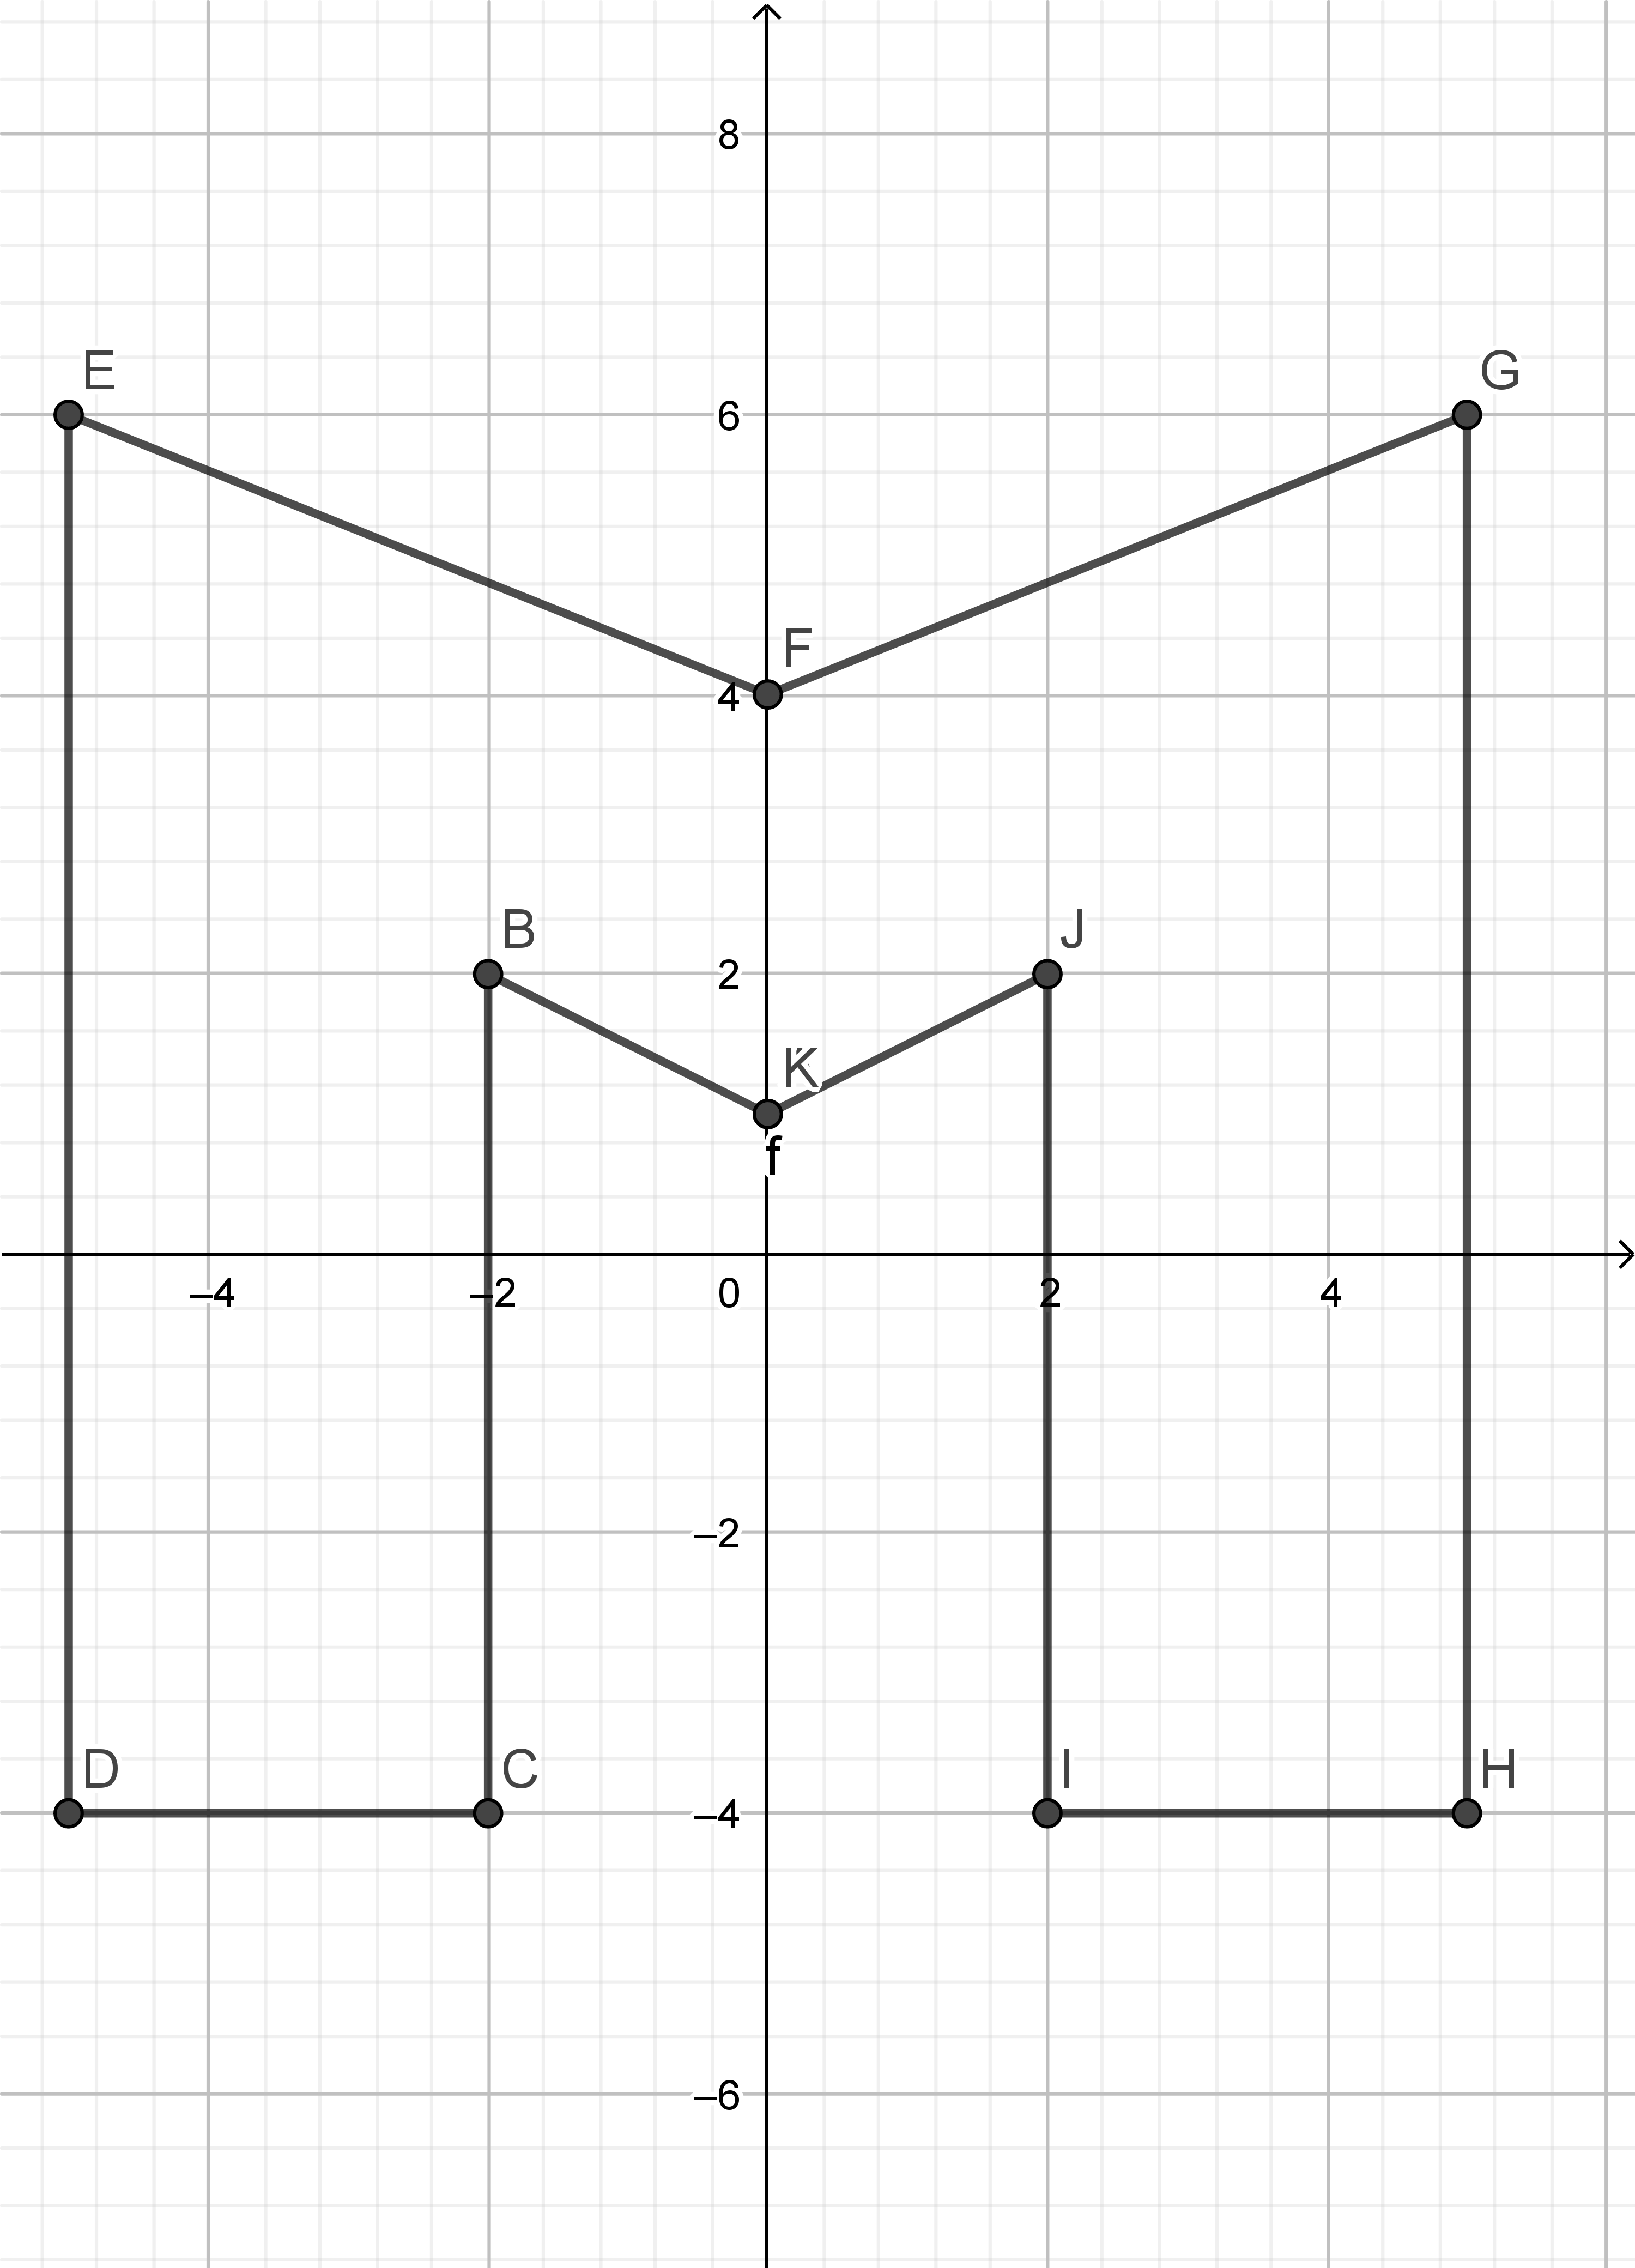
\includegraphics[width=60mm]{./images/ex3-letra-inicial.png}
                \caption{Letra inicial}
            \end{figure}
    
        \item
            Para a reflexão em torno do eixo y, usaremos
            \begin{equation}
                \begin{bmatrix} 
                -1 & 0 \\
                 0 & 1
                \end{bmatrix} 
                \cdot M = 
                \begin{bmatrix} 
                0 & 2 & 2 & 5 & 5 & 0 & -5  & -5 & -2 & -2 & 0 \\
                1 & 2 & -4&-4 & 6 & 4 & 6   & -4 & -4 &  2 & 1
                \end{bmatrix} 
            \end{equation}
        \item
            Para a o cisalhamento na horizontal, usaremos
            \begin{equation}
                \begin{bmatrix} 
                1 & 1/2 \\
                 0 & 1
                \end{bmatrix} 
                \cdot M = 
                \begin{bmatrix} 
                1/2 & -1 & -4 & -7 & -2 & 2 & 8  & 3 & 0 & 3 & 1/2 \\
                1 & 2 & -4&-4 & 6 & 4 & 6   & -4 & -4 &  2 & 1
                \end{bmatrix} 
            \end{equation}
            \begin{figure}[ht!]
                \centering
                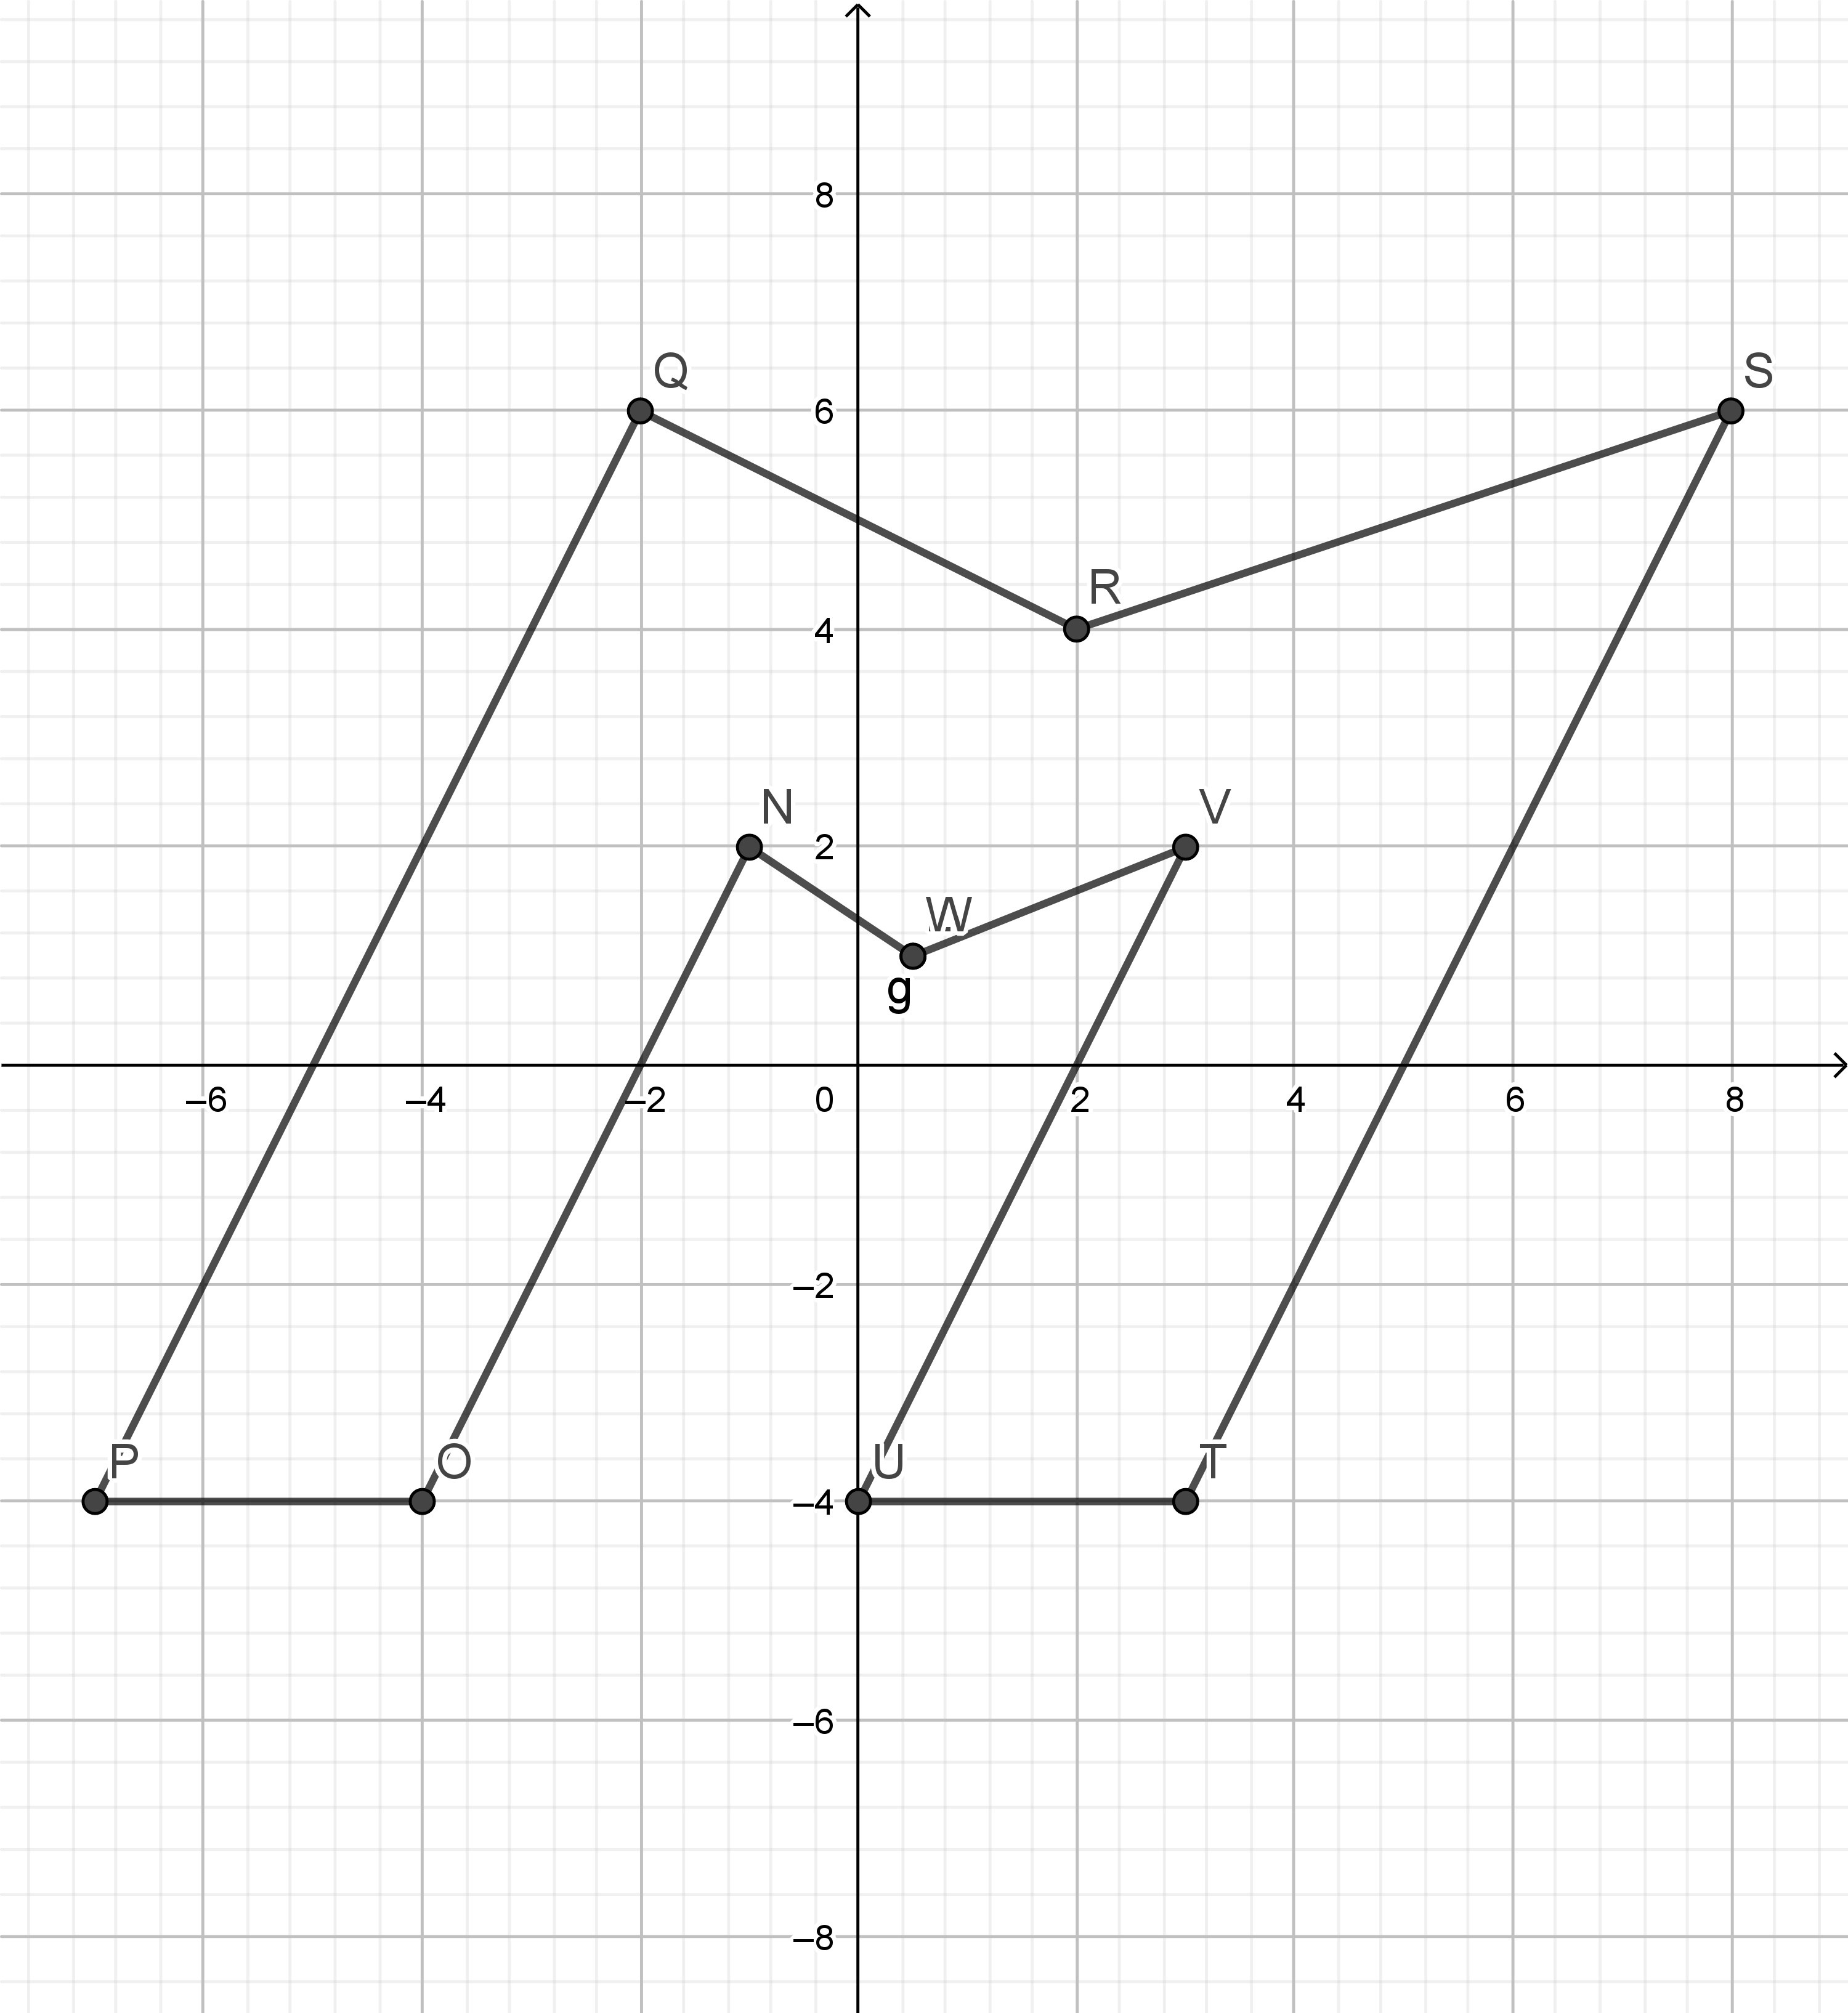
\includegraphics[width=60mm]{./images/ex3-cisalhamento.png}
                \caption{Cisalhamento na horizontal}
            \end{figure}

        \item 
            Para a reflexão em torno da reta $y = 3x$ primeiramente escolheremos uma base
            conveniente e verificaremos qual a imagem dos vetores da base. 
            Escolheremos a base $\beta = \{(1;3) ; (1;0)\}$, cujas imagens são: \\
            $(1;3) \rightarrow (1,3)$ \\
            $(1;0) \rightarrow (x_0; y_0)$ \\
            Sejam \\
            $f: \mathbb{R} \rightarrow \mathbb{R} ; f(x) = 3x$ e \\
            $g: \mathbb{R} \rightarrow \mathbb{R} ; g(x) = -3^{-1}x + b = \dfrac{-1}{3}x + b$ \\
            assim $f$ é a reta de reflexão e $g$ é uma função auxiliar. A ideia é que a reflexão
            de um ponto digamos, $P_1$, em torno de uma reta estará situado sobre a reta definida 
            pelos pontos $P_1$ e o pé da perpendicular ($P_2$) de $P_1$ em nossa reta, no caso $f$. \\
			\begin{tikzpicture}
                \draw[gray] (-2,2) grid[xstep=1, ystep=1]  (2,-2);
                \fill (1,0)  circle[radius=2pt];
                \node[below=3pt of {(1,0)}, outer sep=2pt,fill=white] {\tiny$ P_1(1,0)$};
                
                \fill (1/10,3/10)  circle[radius=2pt];
                \node[above right=2pt of {(1/10,3/10)}, outer sep=2pt,fill=white] {\tiny $P_2(\frac{1}{10},\frac{3}{10})$};

                \fill (-8/10,6/10)  circle[radius=2pt];
                \node[above=3pt of {(-8/10,6/10)}, outer sep=2pt,fill=white] {\tiny $P_3(\frac{-8}{10},\frac{6}{10})$};

                \draw[->][black] (-2,0) -- (2,0) node[right] {$x$};
                \draw[->][black] (0,-2) -- (0,2) node[above] {$y$};

                \draw[scale=1,domain=-7/10:7/10,smooth,variable=\x,blue] plot ({\x},{3 *\x});
                \node[below=2pt of {(0.7,2)}, outer sep=2pt, color=blue] {\tiny $f$};

                \draw[scale=1,domain=-2:2,smooth,variable=\x,red] plot ({\x},{-1/3 *\x + 1/3});
                \node[below=2pt of {(-0.7,0.5)}, outer sep=2pt, color=red] {\tiny $g$};

			\end{tikzpicture} \\
            Ainda, $P_3$ é tal que $P_2$ seja o ponto médio de $P_1$ e $P_3$, 
            logo $P_3 = (\frac{1}{10} - \abs{1-\frac{1}{10}} ; y) = \Big( \frac{-8}{10} ; g(\frac{-8}{10}) \Big) = \Big( \frac{-8}{10} ; \frac{6}{10} \Big)$.
            O coeficiente angular de $g$ obtemos facilmente lembrando que no caso de funções que descrevem retas, 
            elas são perpendiculares se, e somente se o produto dos coeficientes lineares for igual a $-1$. O coeficiente linear obtemos
            usando o coeficiente angular com o ponto $P_1$. Com isso obtemos $g(x) = \frac{-1}{3}x+\frac{1}{3}$. $P_2$ 
            é a intersecção das duas retas, logo:
            \begin{equation}
                f(x) = g(x) \iff
                3x = \frac{-1}{3} x + \frac{1}{3} \iff
                x = \frac{1}{10}
            \end{equation}
            Ainda, $P_2 = (\frac{1}{10}, f(\frac{1}{10}) ) = (\frac{1}{10};\frac{3}{10})$
            Agora encontremos os coeficientes da matriz tranformação:
            \begin{equation}
                \begin{bmatrix}
                a & b \\
                c & d \\
                \end{bmatrix}
                \cdot
                \begin{bmatrix}
                1 \\
                3 \\
                \end{bmatrix}
                =
                \begin{bmatrix}
                1 \\
                3 \\
                \end{bmatrix}
            \end{equation}
            \begin{equation}
                \begin{bmatrix}
                a & b \\
                c & d \\
                \end{bmatrix}
                \cdot
                \begin{bmatrix}
                1 \\
                0 \\
                \end{bmatrix}
                =
                \begin{bmatrix}
                \frac{-8}{10} \\
                \frac{6}{10} \\
                \end{bmatrix}
            \end{equation}
            Chegamos ao sistema:

            \systeme*{{a + 3b = 1}, {c + 3d = 3}, {a = \frac{-8}{10}}, {c = \frac{6}{10}}} \\
            Resolvendo chegamos na matriz:
            \begin{equation}
            \begin{bmatrix}
                \frac{-8}{10} & \frac{3}{5} \\
                \frac{6}{10} & \frac{4}{5} \\
            \end{bmatrix}
                \iff T(x;y) = \Big( \frac{-8}{10}x + \frac{3}{5}y ; \frac{6}{10}x + \frac{4}{5}y \Big)
            \end{equation}
            \begin{figure}[ht!]
                \centering
                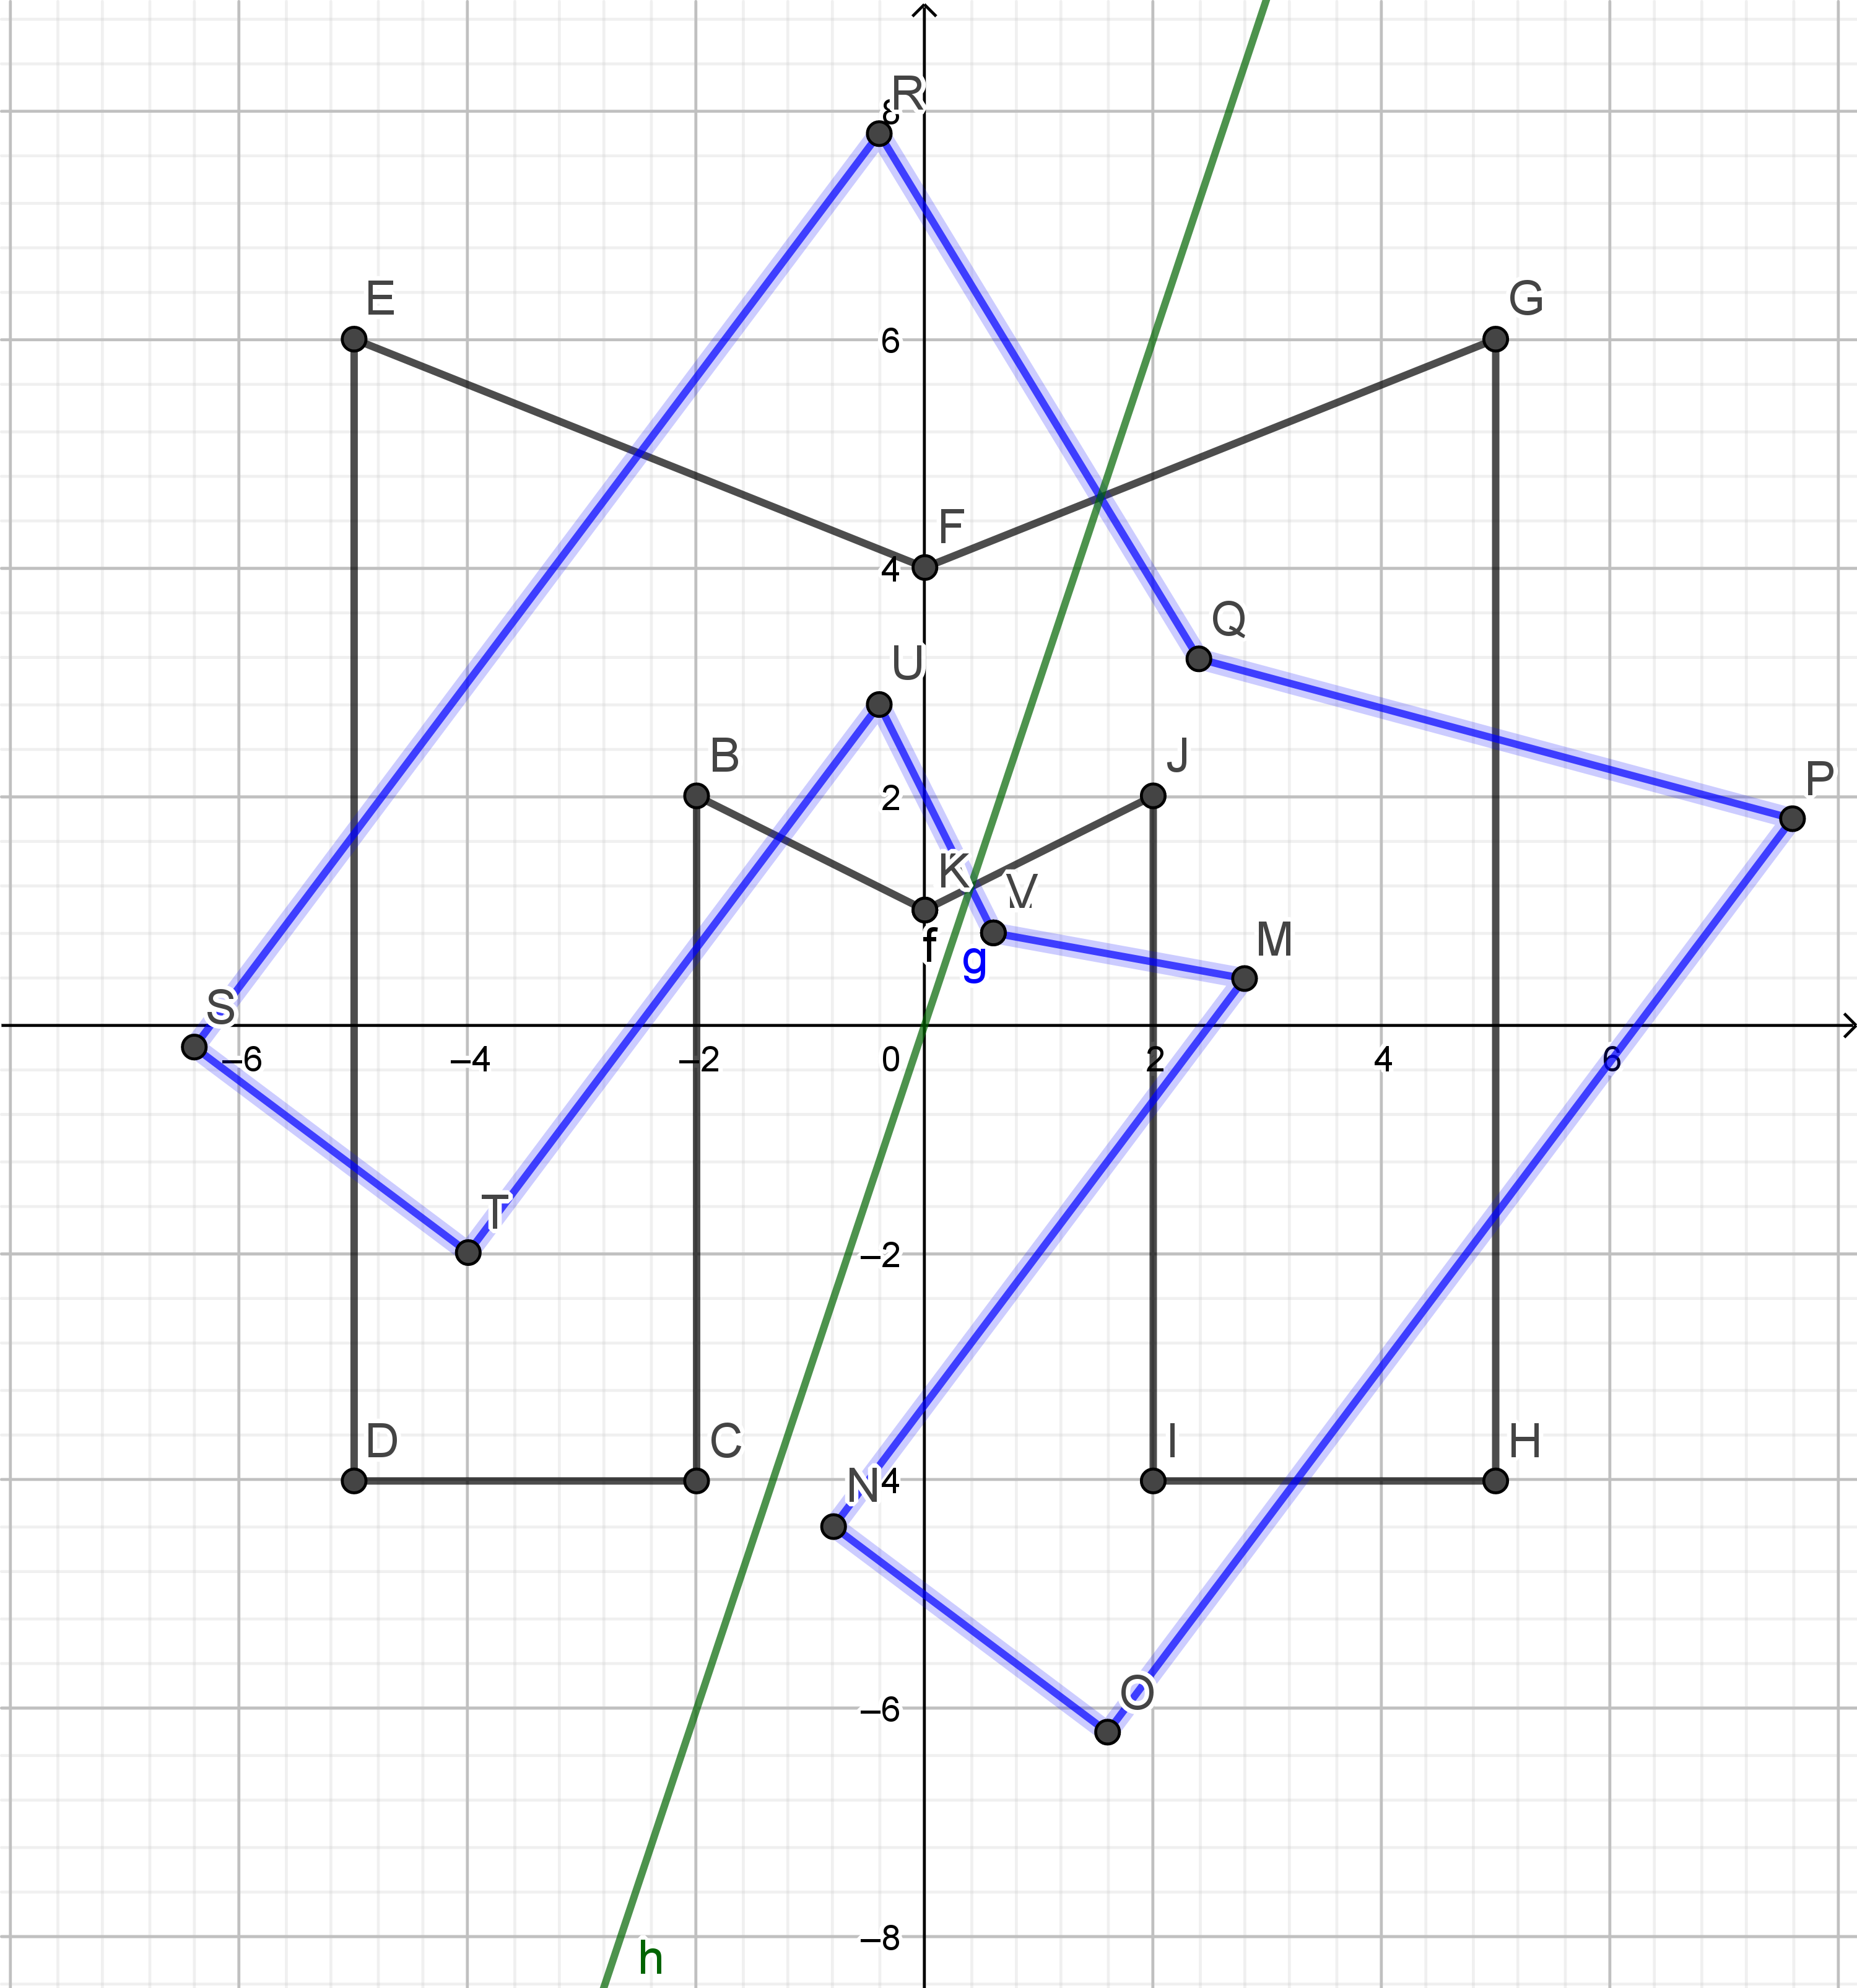
\includegraphics[width=80mm]{./images/ex3-c-c-reflexao-na-reta.png}
                \caption{Reflexão em torno de $y=3x$}
            \end{figure}
        \end{enumerate}

    \item
        \begin{enumerate}
            \item
                Considerando os pontos $B, E$ temos:\\
                $T(E) = T(0;2) = (2;6) \\
                 T(B) = T(1;-1) = (2; -2)$

                \begin{equation}
                    \begin{bmatrix}
                    a & b \\
                    c & d \\
                    \end{bmatrix}
                    \cdot
                    \begin{bmatrix}
                    0 \\
                    2 \\
                    \end{bmatrix}
                    =
                    \begin{bmatrix}
                    2 \\
                    6
                    \end{bmatrix}
                \end{equation}
                \begin{equation}
                    \begin{bmatrix}
                    a & b \\
                    c & d \\
                    \end{bmatrix}
                    \cdot
                    \begin{bmatrix}
                    1 \\
                    -1 \\
                    \end{bmatrix}
                    =
                    \begin{bmatrix}
                    2 \\
                    -2
                    \end{bmatrix}
                \end{equation}
                Chegamos ao sistema:
                \systeme*{{2b = 1}, {2d = 6}, {a = 3}, {c = 1}} \\
                \begin{equation}
                    \begin{bmatrix}
                        a&b \\
                        c&d \\
                    \end{bmatrix}
                    =
                    \begin{bmatrix}
                        3&1 \\
                        1&3 \\
                    \end{bmatrix}
                    \iff T(x;y) = (3x+y ; x+3y)
                \end{equation}
            \item
                \begin{equation}
                    \begin{bmatrix}
                        3 - \lambda & 1 \\
                        1 & 3 - \lambda \\
                    \end{bmatrix}
                    = Z \leadsto \\
                    det Z = (3 - \lambda)^2 -1 = (\lambda -2)(\lambda -4)
                \end{equation}
                Logo os autovalores são $\{2, 4\}$, pois zeram o polinômio característico.
                \begin{equation}
                    \begin{bmatrix}
                        3 - 2 & 1 \\
                        1 & 3 - 2 \\
                    \end{bmatrix}
                    =
                    \begin{bmatrix}
                        1 & 1 \\
                        1 & 1 \\
                    \end{bmatrix}
                    \leadsto 
                    \begin{bmatrix}
                        1 & 1 \\
                        1 & 1 \\
                    \end{bmatrix}
                    \begin{bmatrix}
                        x \\
                        y
                    \end{bmatrix}
                    \begin{bmatrix}
                        0 \\
                        0
                    \end{bmatrix}
                    \implies x + y = 0 \leadsto \beta_{\lambda=2} = \{(1;-1)\}
                \end{equation}

                \begin{equation}
                    \begin{bmatrix}
                        3 - 4 & 1 \\
                        1 & 3 - 4 \\
                    \end{bmatrix}
                    =
                    \begin{bmatrix}
                        -1 & 1 \\
                        1 & -1 \\
                    \end{bmatrix}
                    \leadsto 
                    \begin{bmatrix}
                        -1 & 1 \\
                        1 & -1 \\
                    \end{bmatrix}
                    \begin{bmatrix}
                        x \\
                        y
                    \end{bmatrix}
                    \begin{bmatrix}
                        0 \\
                        0
                    \end{bmatrix}
                    \implies x - y = 0 \leadsto \beta_{\lambda=4} = \{(1;1)\}
                \end{equation}
                Assim, os autovetores (que $T(u)$ ficam na mesma direção que $u$) são múltiplos de $(1;-1)$ ou múltiplos de $(1;1)$,
                e ficam ampliados ou reduzidos pelo módulo do autovalor correspondente (autovalor que nos permitiu encontrar a base).
                E o sentido varia de acordo com o sinal do autovalor.
            \item
            \begin{figure}[ht!]
                \centering
                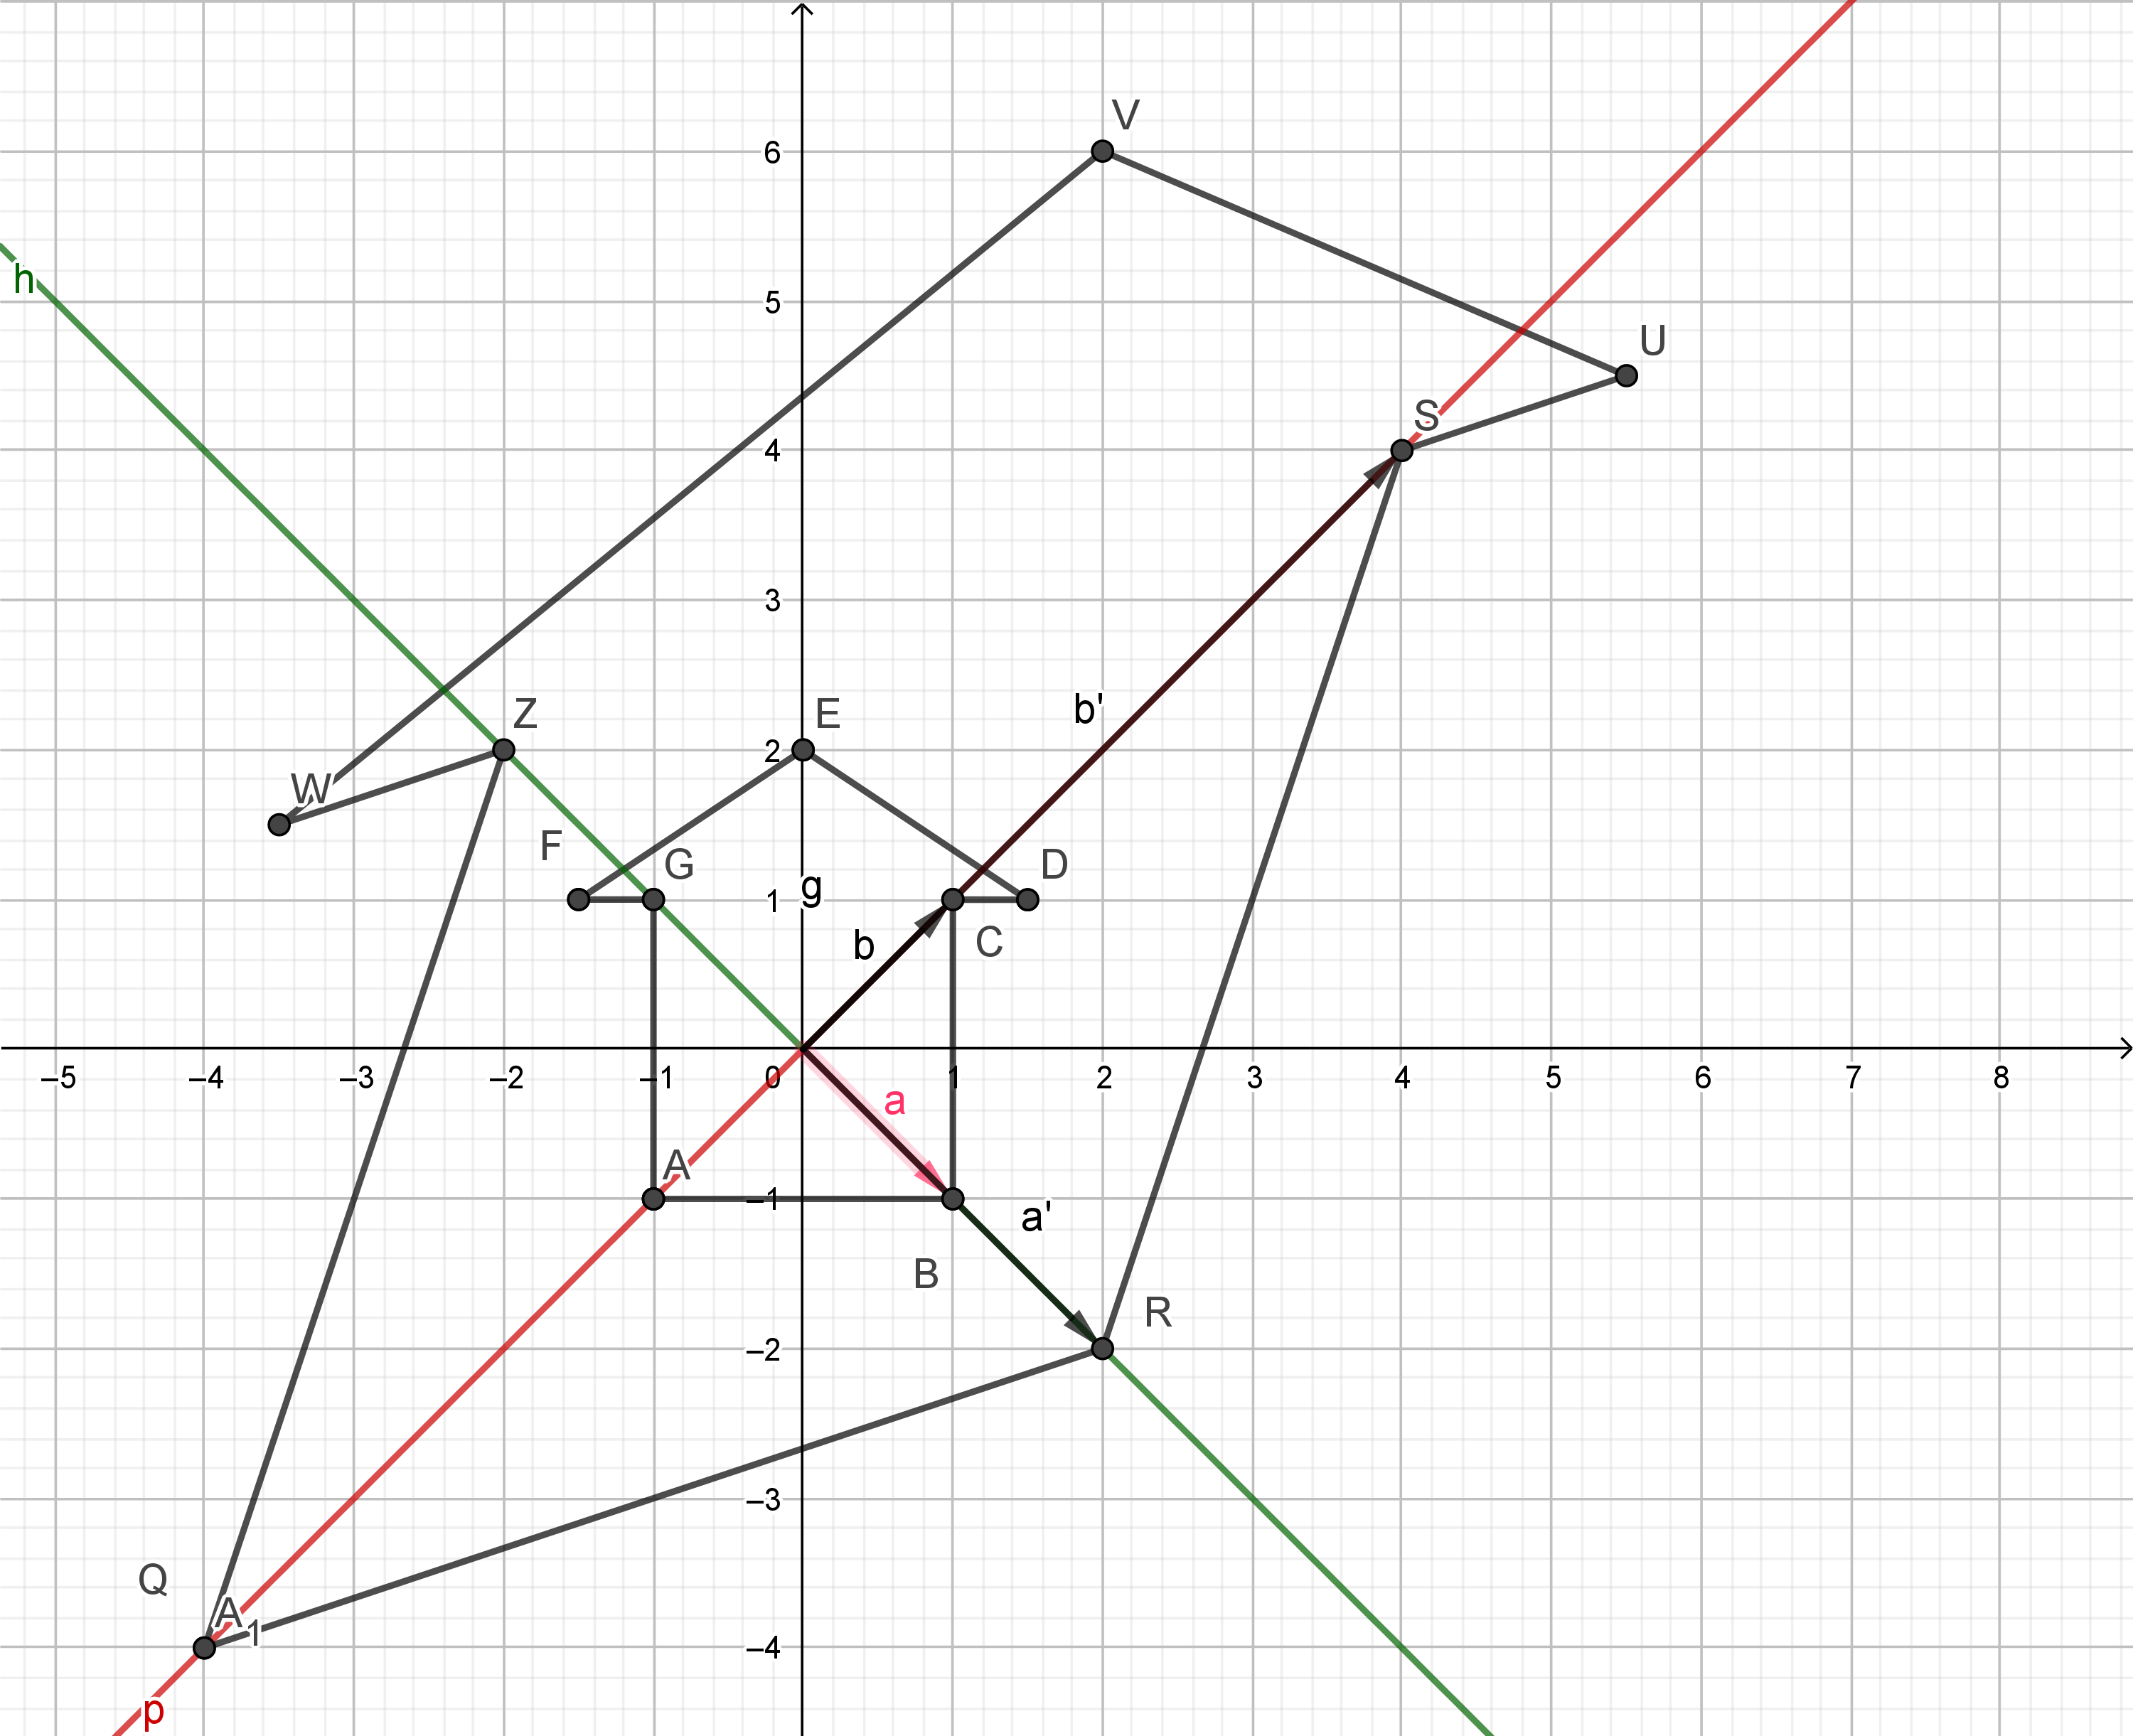
\includegraphics[width=100mm]{./images/ex4-final.png}
                \caption{Representação da transformação e autovetores}
            \end{figure}
            Os vetores nas retas $p, h$ são transformados em vetores que tem a mesma direção dos vetores iniciais. Por exemplo,
            $T(a) = a'$ e $T(b) = b'$. Peguei vetores de cada base mas poderia ter pego qualquer multiplo que estivessem sobre $p$ ou $h$.

        \end{enumerate}
\end{enumerate}
\end{document}

